\chapter{Solving DSGE models - basics} \label{ch:solbase}

This chapter focusses on the solution of DSGE models. The term ``solution'' is used rather broadly to encompass a wide spectrum of functionalities and user needs. This chapter should be relevant if you're interested in solving a system of first order and equilibrium conditions for a set of endogenous variables. You may also be interested in how this system behaves in response to shocks, whether expected or stochastic, temporary or permanent. Likewise, you may want to explore how the system comes back to its steady state or moves to a new one. We recommend that you read this chapter chronologically, as its goal is to get you to write a typical Dynare input file and obtain basic results. More advanced features and possible customization are discussed in chapter \ref{ch:soladv}.

\section{Introducing an example}
The goal of this first section is to introduce a simple example right off the bat, in order to give a more tangible context in which to introduce the relevant Dynare features and commands.\\

The model is a simplified standard RBC model taken from \citet{CollardJuillard2003} which served as the original User Guide for Dynare. Other examples along the same lines (from the most basic to more intricate RBC models) with helpful notes and explanations, are provided by Jesus Fernandez-Villaverde in the \href{http://www.cepremap.cnrs.fr/juillard/mambo/index.php?option=com_content&task=category&sectionid=11&id=96&Itemid=89}{official examples} section of the Dynare website. \\

The economy consists of an infinitely living representative agent who values consumption $c_t$ and labor services $h_t$ according to the following utility function
\[
\mathbb{E}_t \sum_{\tau=t}^\infty \beta^{\tau-t} \left( \log (c_t) - \theta \frac{h_t^{1+\psi}}{1+\psi} \right)
\] 
where, as usual, the discount factor $0<\beta<1$, the disutility of labor $\theta > 0$ and the labor supply elasticity $\psi \geq 0$. \\

A social planner maximizes this utility function subject to the budget constraint
\[
c_t + i_t = y_t
\]
where $i_t$ is investment and $y_t$ output. Consumers are therefore also owners of the firms. The economy is a real economy, where part of output can be consumed and part invested to form physical capital. As is standard, the law of motion of capital is given by
\[
k_{t+1} = \exp (b_t)i_t + (1-\delta)k_t
\]
with $0<\delta<1$, where $\delta$ is physical depreciation, $\alpha$ the capital elasticity in the production function and where $b_t$ is a shock affecting incorporated technological progress. \\

We assume output is produced according to a standard constant returns to scale technology of the form
\[
y_t = \exp (a_t)k_t^\alpha h_t^{1-\alpha}
\]
with $0<\alpha<1$, and where $a_t$ represents a stochastic technological shock (or Solow residual). \\

Finally, we specify a \textbf{shock structure} that allows for shocks to display persistence across time and correlation in the current period. That is
\[
\left( \begin{array}{c}a_t \\
b_t \end{array} \right) = \left( \begin{array}{c c} \rho & \tau \\
\tau & \rho \end{array} \right) \left( \begin{array}{c}a_{t-1} \\
b_{t-1} \end{array} \right) + \left( \begin{array}{c}\epsilon_t \\
\nu_t \end{array} \right)
\]
where $|\rho + \tau|<1$ and $|\rho - \tau|<1$ to ensure stationarity (we call $\rho$ the coefficient of persistence and $\tau$ that of cross-persistence). Furthermore, we assume $\mathbb{E}_t (\epsilon_t)=0$, $\mathbb{E}_t (\nu_t)=0$ and that the contemporaneous variance-covariance matrix of the innovations $\epsilon_t$ and $\nu_t$ is given by
\[
\left( \begin{array}{c c} \sigma_\epsilon^2 & \psi \sigma_\epsilon \sigma_\nu \\
\psi \sigma_\epsilon \sigma_\nu & \sigma_\nu^2 \end{array} \right)
\]
and where $corr(\epsilon_t \nu_s)=0$, $corr(\epsilon_t \epsilon_s)=0$ and $corr(\nu_t \nu_s)=0$ for all $t \neq s$. \\

This system - probably quite similar to standard RBC models you have run into - yields the following first order conditions (which are straightforward to reproduce in case you have doubts\ldots) and equilibrium conditions drawn from the description above. Note that the first equation captures the labor supply function and the second the intertemporal consumption Euler equation.
\[
\begin{aligned}
c_t \theta h_t^{1+\psi} = (1-\alpha)y_t \\
1= \beta \mathbb{E}_t \left[ \left( \frac{\exp(b_t)c_t}{\exp(b_{t+1})c_{t+1}} \right) \left( \exp(b_{t+1}) \alpha \frac{y_{t+1}}{k_{t+1}}+1-\delta \right) \right] \\
y_t = \exp (a_t)k_t^\alpha h_t^{1-\alpha} \\
k_{t+1} = \exp (b_t)i_t + (1-\delta)k_t \\
a_t = \rho a_{t-1} + \tau b_{t-1} + \epsilon_t \\
b_t = \tau a_{t-1} + \rho b_{t-1} + \nu_t
\end{aligned}
\] 

Alternatively, for reasons that will become evident later, the system is simple enough that we can use pen and paper to linearize it by hand. This yields the following equations where hats over variables imply percent deviation from steady state and variables without time subscript correspond to steady state values. (** check problems with equations)
\[
\begin{aligned}
\hat{c}_t + (1+\psi) \hat{h}_t = \hat{y}_t \\
\hat{c}_t =  \mathbb{E}_t \hat{c}_{t+1} - (1-\beta + \delta \beta) \mathbb{E}_t \left[ \hat{y}_{t+1} - \hat{k}_{t+1} \right] \\
\hat{y}_t = \alpha \hat{k}_t + (1-\alpha) \hat{h}_t \\
\mathbb{E}_t \hat{k}_{t+1} = \frac{1}{\alpha}\left(\frac{1}{\beta}-1+\delta \right) \hat{y}_t - \frac{c}{k} \hat{c}_t + (1-\delta)\hat{k}_t \\
\hat{a}_t = \rho \hat{a}_{t-1} + \tau \hat{b}_{t-1} + \hat{\epsilon}_t \\
\hat{b}_t = \tau \hat{a}_{t-1} + \rho \hat{b}_{t-1} + \hat{\nu}_t
\end{aligned}
\] 
This ends the exposition of the example. Now, let's roll up our sleeves and see how we can get the model into Dynare and actually generate some impulse response functions. 

\section{Dynare .mod file structure}
Input into Dynare involves the .mod file, as mentioned loosely in the introduction of this Guide. The .mod file can be written in any editor, external or internal to Matlab. It will then be read by Matlab by first navigating within Matlab to the directory where the .mod file is stored and then by typing in the Matlab command line \texttt{Dynare filename.mod;} (although actually typing the extension .mod is not necessary). But before we get into executing a .mod file, let's start by writing one! \\

It is convenient to think of the .mod file as containing four distinct parts, illustrated in figure \ref{fig:modstruct}:
\begin{itemize}
\item preamble: lists variables and parameters
\item model: spells out the model
\item dynamics: gives indications to find the steady state and defines the shocks to the system
\item computation: asks to undertake specific operations (e.g. forecasting, estimating impulse response functions)
\end{itemize}
Our exposition below will follow these distinctions. 
\begin{figure} \label{fig:modstruct}
\begin{center} 
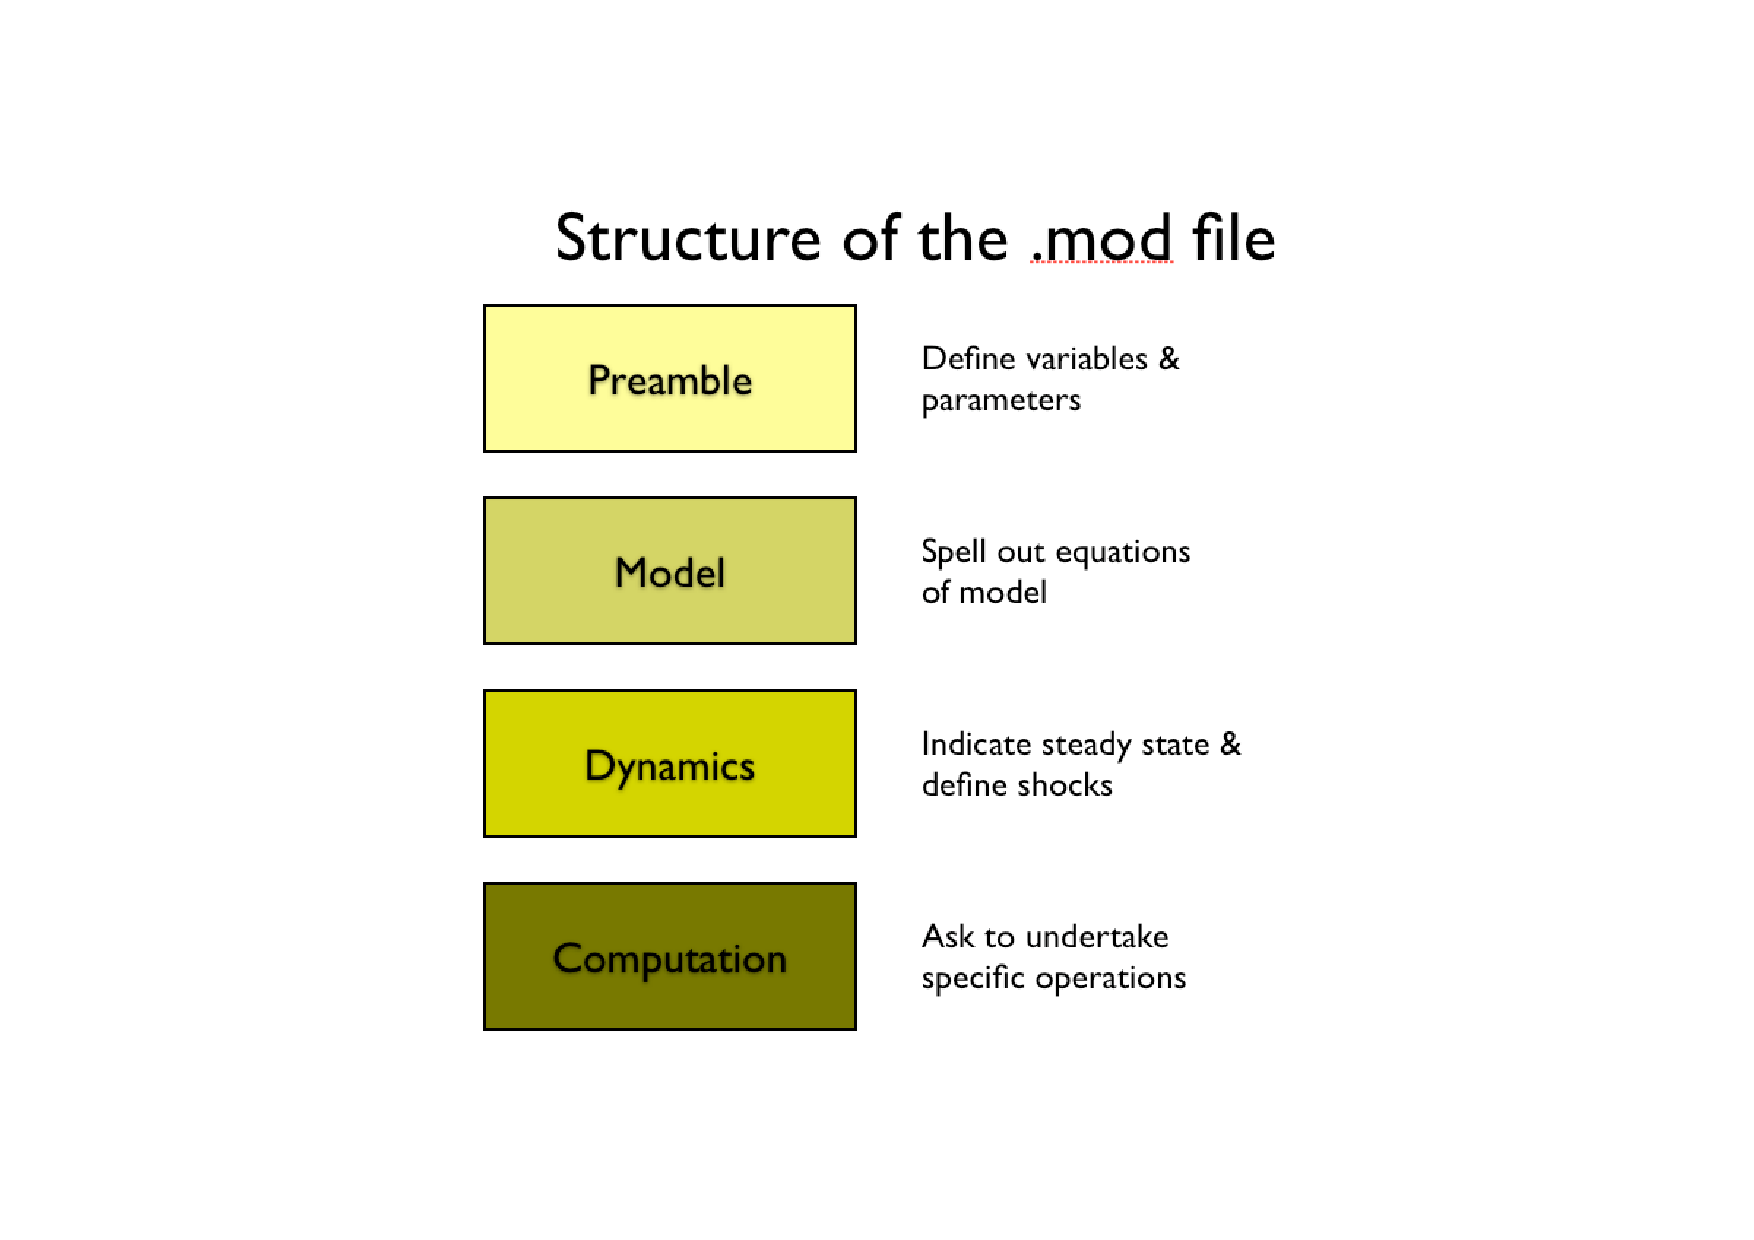
\includegraphics[width=1.0\textwidth]{P_ModStruct2} 
\end{center} 
\caption[Structure of the .mod file]{The .mod file contains four logically distinct parts.} 
\end{figure}

\section{Filling out the preamble}
The preamble generally involves three commands that tell Dynare what are the model's variables, which are endogenous and what are the parameters. The \textbf{commands} are:
\begin{itemize}
\item \texttt{var} starts the list of endogenous variables, to be separated by commas. 
\item \texttt{varexo} starts the list of exogenous variables that will be shocked.
\item \texttt{parameters} starts the list of parameters and assigns values to each.
\end{itemize}

In the case of our example, here's what the \textbf{preamble would look like}:\\ 
\\
\texttt{var y, c, k, a, h, b;\\
varexo e,u;\\
parameters beta, rho, beta, alpha, delta, theta, psi, tau;\\
alpha = 0.36;\\
rho   = 0.95;\\
tau   = 0.025;\\
beta  = 0.99;\\
delta = 0.025;\\
psi   = 0;\\
theta = 2.95;\\
phi   = 0.1;}\\

As you can tell, writing a .mod file is really quite straightforward. Two quick comments: \textsf{\textbf{TIP!}} Remember that each line of the .mod file must be terminated by a semicolon (;). To comment out any line, start the line with two forward slashes (//).  

\section{Specifying the model} \label{sec:modspe}
\subsection{Model in Dynare notation}
One of the beauties of Dynare is that you can input your model's equations almost as if you were writing them to communicate them to a person - not a machine. No fancy transformations, no matrix manipulations, no ambiguous deliberations about the backward or forward looking nature of variables are necessary. Dynare's pre-processor does all the grunt work to build and populate the various matrices necessary to untangle and solve the system. Let's first have a look at our model in Dynare notation, and then take a moment to point out some of its important features. \\
\\
\texttt{model;\\
c*theta*h$\hat{ }$(1+psi)=(1-alpha)*y;\\
k = beta*(((exp(b)*c)/(exp(b(+1))*c(+1)))\\
    *(exp(b(+1))*alpha*y(+1)+(1-delta)*k));\\
y = exp(a)*(k(-1)$\hat{ }$alpha)*(h$\hat{ }$(1-alpha));\\
k = exp(b)*(y-c)+(1-delta)*k(-1);\\
a = rho*a(-1)+tau*b(-1) + e;\\
b = tau*a(-1)+rho*b(-1) + u;\\
end;}\\

\subsection{Some commands and conventions}
The above example illustrates the use of a few important commands and conventions to translate a model into a Dynare-readable .mod file. 
\begin{itemize}
\item The first thing to notice, is that the model block of the .mod file begins with the command \texttt{model} and ends with the command \texttt{end}. 
\item Second, in between, there need to be as many equations as you declared endogenous parameters (this is actually one of the first things that Dynare checks; it will immediately let you know if there are any problems). 
\item Third, as in the preamble and everywhere along the .mod file, each line ends with a semicolon (except when a line is too long and you want to break it across two lines). 
\item Fourth, equations are entered one by one, with the same variable and parameter names as declared in the preamble. 
\item Fifth, the specification of the equations looks almost identical to those listed as the first order conditions above, except for a few important differences. These make up the variable input conventions and are listed in the box below for greater clarity.
\end{itemize}

\begin{tabular}{|p{11cm}|}
\hline
\textbf{Variable input conventions}\\
\begin{enumerate}
\item Variables entering the system with a time $t$ subscript are written plainly. For example, $x_t$ would be written $x$. 
\item Variables entering the system with a time $t-n$ subscript are written with $(-n)$ following them. For example, $x_{t-2}$ would be written $x(-2)$ (incidentally, this would count as two backward looking variables). 
\item In the same way, variables entering the system with a time $t+n$ subscript are written with $(+n)$ following them. For example, $x_{t+2}$ would be written $x(+2)$.
\item The only slight complications has to do with stock variables. One rule that may help is: in Dynare, the timing of each variable reflects when that variable is decided. For instance, our capital stock today is not decided today, but yesterday (recall, it is a function of yesterday's investment and capital stock). Thus, we would write it with a lag, meaning that the $k_{t+1}$ in our model equations gets reported into the .mod file as $k$ (at time $t$).
\item A slightly more roundabout way to explain the same thing is that for stock variables, you must use a ``stock at the end of the period'' concept. It is investment during period $t$ that sets stock at the end of period $t$. Be careful, a lot of papers use the ``stock at the beginning of the period'' convention. For instance, in some wage negociation models, wages used during a period are set the period before. In the equation for wages, you can write wage in period $t$ (when they are set), but in the labor demand equation, wages should appear with a one period lag. 
\end{enumerate}
\\
\hline
\end{tabular}\\
\\

\subsection{Predetermined vs. non-predetermined variables}
What does all this mean for predetermined vs. non-predetermined variables? If you are used to solving simple DSGE models by hand, or to inputting the matrices corresponding to your equations, you are probably eagerly waiting for an answer. \textsf{\textbf{TIP!}} Actually, you may surprised (relieved?!) to know that Dynare figures out automatically which variables are predetermined and non-predetermined. Especially in more complicated models, the categorization of variables can be difficult, if not ambiguous, and a source of much frustration.\\ 

In Dynare, a forward-looking variable is a variable that appears in the model with a lead. For example, $c(+1)$.  A predetermined variable is a variable that appears with a lag. Note that a variable can be both forward-looking and predetermined. A static variable is a variable that appears in the model with neither a lead or a lag.\\

\subsection{Linear and log-linearized models}
There are two other variants of the system's equations which Dynare accommodates. First, the \textbf{linear model} and second, the \textbf{model in exp-logs}. In the first case, all that is necessary is to write the term \texttt{(linear)} next to the command \texttt{model}. In our example, this would yield the following for the first two lines:\\

** complete once the fixed problem with linearized equations\\

Otherwise, you may be interested to have Dynare take Taylor series expansions in logs rather than in levels. If so, simply rewrite your equations by taking $\exp$ and $\log$ of each variable. The Dynare input convention makes this very easy to do. Our example would need to be re-written as:\\
\\
\texttt{model;\\
exp(c)*theta*exp(h)$\hat{ }$(1+psi)=(1-alpha)*exp(y);\\
exp(k) = beta*(((exp(b)*exp(c))/(exp(b(+1))*exp(c(+1))))\\
         *(exp(b(+1))*alpha*exp(y(+1))+(1-delta)*exp(k)));\\
exp(y) = exp(a)*(exp(k(-1))$\hat{ }$alpha)*(exp(h)$\hat{ }$(1-alpha));\\
exp(k) = exp(b)*(exp(y)-exp(c))+(1-delta)*exp(k(-1));\\
a = rho*a(-1)+tau*b(-1) + e;\\
b = tau*a(-1)+rho*b(-1) + u;\\
end;}\\
so that the levels of variables are given by $\exp(variable)$.\\

\subsection{Taking advantage of Matlab}
(\textbf{\textsf{TIP!}}) Dynare accepts standard Matlab expressions in any of the model equations. The only thing you need to do is to start the line with \# and then enter the Matlab command as you would normally. For example, if you want to define a variable in terms of another, you can write \texttt{\# b = 1 / c}. This feature, actually, is more useful when carrying out model estimation and wanting to declare transformations of parameters. 

\section{Specifying dynamics (steady states and shocks)}
In the ``dynamics'' block of the .mod file, you need to specify two things: steady state values and shocks to the exogenous variables; basically, where is your model starting from (steady state, usually) and where is it going (due to the shocks)? Let's briefly describe the relevant commands and then worry about how to mix and match them depending on the type of shock you want to create and the type of model you're dealing with.\\

\subsection{Specifying steady states}
To specify steady states, you use the commands \texttt{initval}, \texttt{endval} or, more rarely, \texttt{histval}. Each command initiates a block which must be terminated by \texttt{end}. In the middle, you should list values for all your variables - endogenous and exogenous (even if the latter is not required for stochastic models, but you may want to get in the habit of doing so anyhow). The \texttt{initval} command allows you to enter your variables' steady state values before any shocks hit the system. Under the \texttt{endval} command, instead, you would list the steady state values to which the system moves after any shocks (assuming the system does not return to its original steady state). Finally, the \texttt{histval} command allows you to specify different historical initial values for different periods, in case you have lagged variables. But because this last command is rarely used, we will not dwell on it; you can instead read more about it in the Reference Manual (** add link). We now focus on the \texttt{intival} block, which is common to all .mod files, and then return later to the \texttt{endval} block, which should be used only in certain circumstances. \\

For our example, here is what the \texttt{initval} block would look like:\\
\\
\texttt{initval;\\
y = 1.08068253095672;\\
c = 0.80359242014163;\\
h = 0.29175631001732;\\
k = 5;\\
a = 0;\\
b = 0;\\
e = 0;\\
u = 0;\\
end;}\\

The difficulty here, of course, is calculating the actual steady state values. Because this is such a central topic, although it borders on a form of art, rather than a science, we've devoted the box below to some \textsf{\textbf{TIPS!}} regarding the calculation of steady states.\\

\begin{tabular}{|p{11cm}|}
\hline
\textbf{Calculating steady states}\\
\\
Suppose, first, that you were interested in entering the exact values of your model's steady states. You could, most straightforwardly, use an external program to calculate these values, like Maple and then enter them by hand. But of course, this procedure could be time consuming and bothersome, especially if you want to alter parameter values. \\

Actually, Dynare can take care of finding your model's steady state by calling the appropriate Matlab functions. To do so, you still need to provide an initial guess of your steady state in the \texttt{initval} block, but you would follow the block with the command \texttt{steady[ \textsl{option} ]}. This will instruct Matlab to use an iterative procedure to find the model's steady state. The procedure itself depends on the option you specify. Possible options are:\texttt{solve\_algo = 0}: uses Matlab Optimization Toolbox FSOLVE; \texttt{solve\_algo = 1}: uses Dynare�s own nonlinear equation solver; and \texttt{solve\_algo = 2}: splits the model into recursive blocks and solves each block in turn. The latter is the default option if none is specified. \\

For complicated models, finding good numerical initial values for the endogenous variables is the trickiest part of finding the equilibrium of that model. Often, it is better to start with a smaller model and add new variables one by one.\\

Unfortunately, for simpler models, you may still run into difficulties in finding your steady state. If so, one option is still available: that of entering your model in linear terms (where variables are expressed in percent deviations from steady state) and thus specifying your steady state values in the \texttt{initval} block as all being zero. \\
\\
\hline
\end{tabular}\\
\\

\subsection{Deterministic vs. stochastic models}
Before we specify shocks, we must decide if our model is deterministic or stochastic. The distinction has actually been a source of significant confusion in the past, so let's try to come to terms with it. The following box defines each type of model:

\begin{tabular}{|p{11cm}|}
\hline
\textbf{Deterministic vs stochastic models}\\
\\
Deterministic models have the following characteristics:
\begin{enumerate}
\item In the recent DSGE literature, deterministic models are somewhat rare. Examples include OLG models without aggregate uncertainty.
\item Models assume full information, perfect foresight, no uncertainty around shocks.
\item Shocks can hit the economy today or at any time in the future, in which case they would be expected with perfect foresight. They can also last one or several periods.
\item Most often, though, models introduce a positive shock today and zero shocks thereafter (with certainty).
\item The solution does not require linearization, as the paths of each variable are fully known.
\item This solution method can therefore be useful when the economy is far away from steady state (when linearizations can provide highly distorted results).
\end{enumerate}\\
Stochastic models, instead, have the following characteristics:
\begin{enumerate}
\item These types of models tend to be more popular in the literature. Examples include most RBC models, or new keynesian monetary models.
\item In these models, shocks hit today (with a surprise), but thereafter their expected value is zero. Thus, these models do not allow for future, expected shocks, nor permanent changes in the exogenous variables.
\item Note that when these models are linearized to the first order, the expectation of the shocks being zero translates into the shocks actually being zero, by certainty equivalence. This is an often overlooked point in the literature which misleads readers in supposing their models may be deterministic.
\item Solutions are technically not simulations (although the literature commonly refers to impulse response functions as being �simulated�). They are instead �solutions� to a constrained maximization problem.
\end{enumerate}
\\
\hline
\end{tabular}\\
\\

\subsection{Adding shocks}
Now let's see how this section's relevant commands - specifying initial and final values, as well as shocks - all fit together depending on the type of model you are using. Figure \ref{fig:shockmodel} summarizes the possible combinations of commands and their usefulness. 
\begin{figure} \label{fig:shockmodel}
\begin{center} 
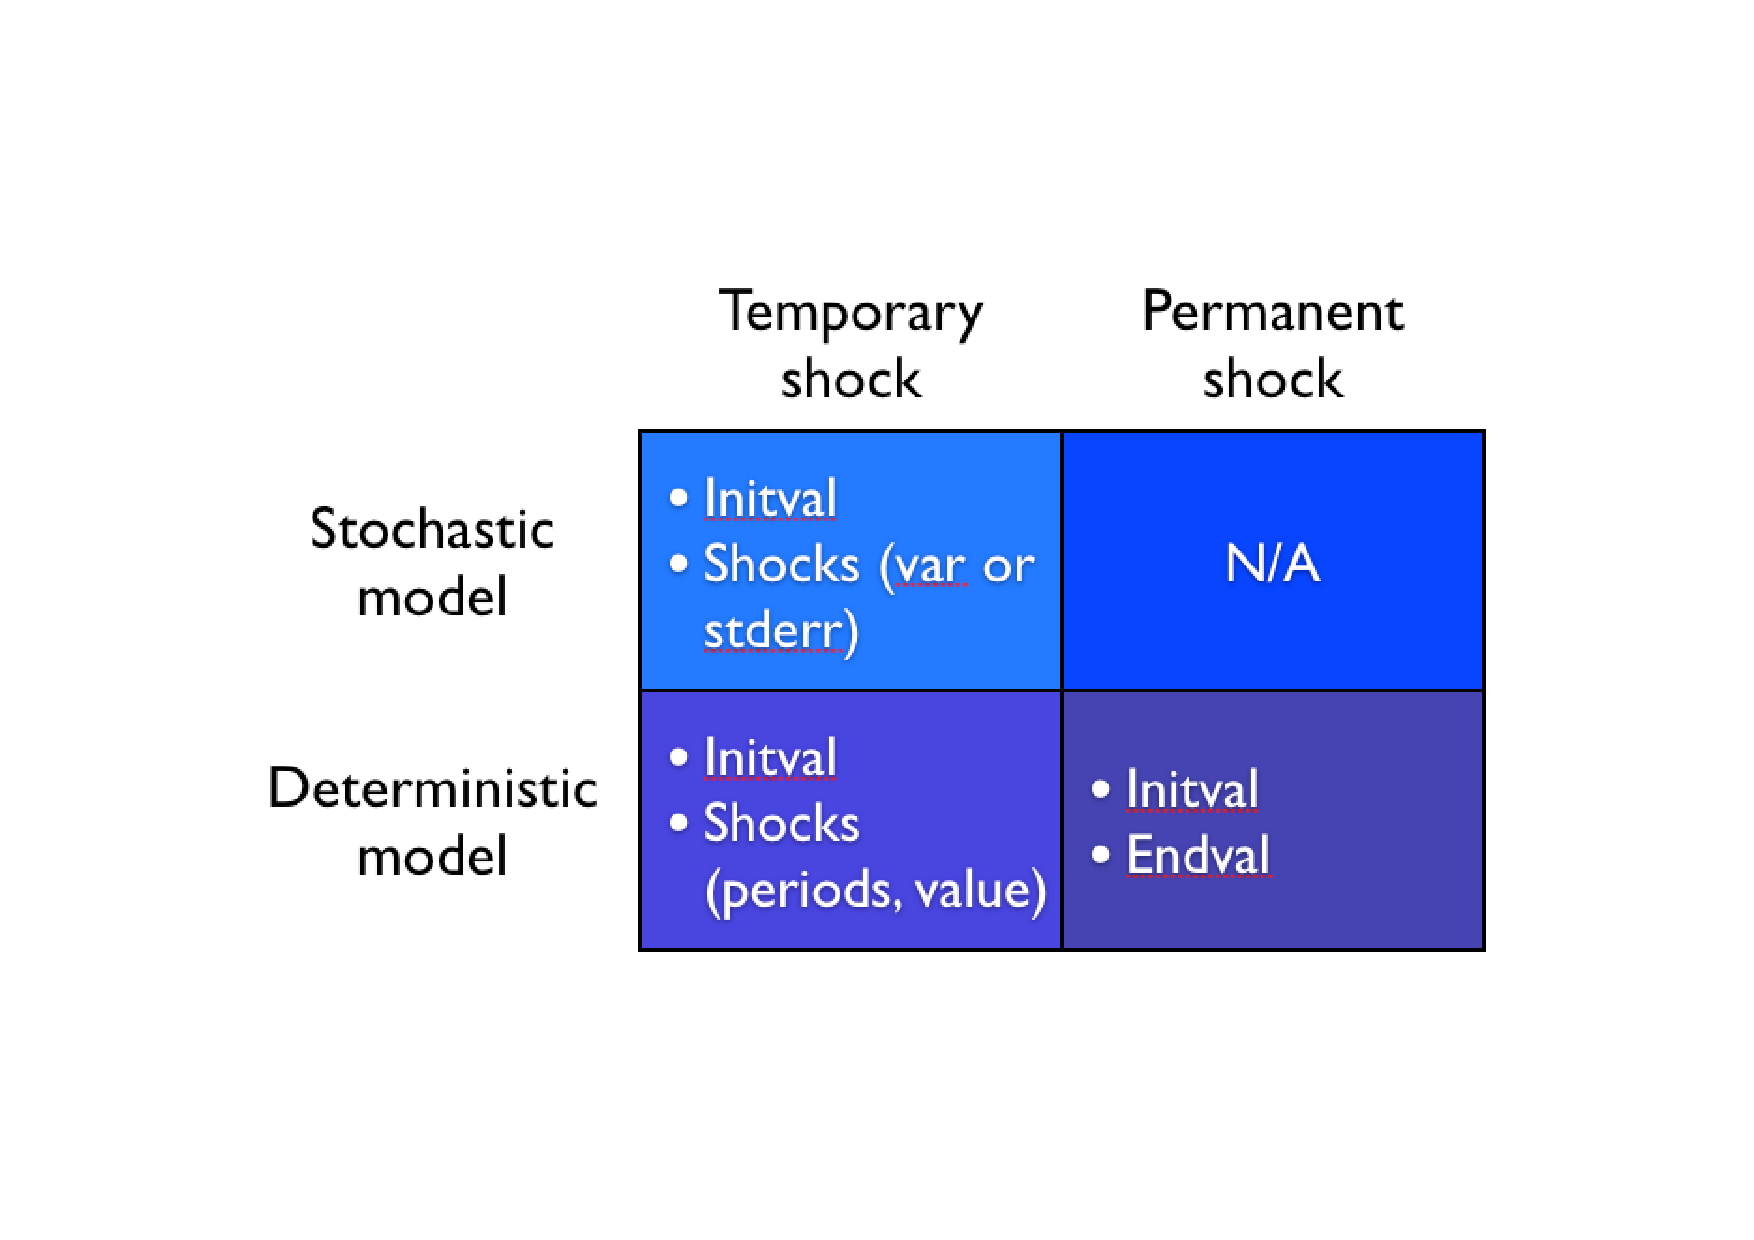
\includegraphics[width=1.0\textwidth]{P_ShockModel2} 
\end{center} 
\caption[Shock and model-type matrix]{Depending on the model type you're working with and the desired shocks, you will need to mix and match the various steady state and shock commands.} 
\end{figure}\\

As seen in the figure, when working with a deterministic model, you have the choice of introducing both temporary and permanent shocks. In the \textbf{deterministic-temporary} case, you are free to set the duration and level of the shock. To specify a shock that lasts 9 periods on $\epsilon_t$, for instance, you would write (** is this a 10\% shock?)\\
\\
\texttt{shocks;\\
var e;
periods 1:9;\\
values 0.1;\\
end;}\\

In the \textbf{deterministic-permanent} case, you would not specify actual ``shocks'', but would simply tell the system to which steady state values you would like it to move to and let Dynare calculate the transition path. To do so, you would use the \texttt{endval} block following the usual \texttt{initval} block. For instance, you may specify all values to remain common between the two blocks, except for the value of the exogenous variable that changes permanently. The example we have used so far is somewhat ill-suited to illustrate this sort of permanent change, since if the exogenous shocks were positive always, they would make the technology variables $a_t$ and $b_t$ explode. Thus, for illustrative purposes, we could imagine getting rid of the last two equations of our system (the equations of motion of the technology variables) as well as the variables $\epsilon_t$ and $\nu_t$, and simply making $a_t$ and $b_t$ exogenous. In that case, we could use the following blocks in our .mod file to introduce a permanent increase in productivity: \\
\\
\texttt{initval;\\
y = 1.08068253095672;\\
c = 0.80359242014163;\\
h = 0.29175631001732;\\
k = 5;\\
a = 0;\\
b = 0;\\
end;\\
\\
endval;\\
y = 1.08068253095672;\\
c = 0.80359242014163;\\
h = 0.29175631001732;\\
k = 5;\\
a = 0.1;\\
b = 0;\\
end;\\
\\
steady;}\\
\\
where the last command \texttt{steady} was added since the \texttt{endval} values are bound to be somewhat imprecise now that we have changed the value of $a_t$. \\

In case of a \textbf{stochastic-temporary} model, which is really what makes most sense for the example introduced earlier, we can only specify a temporary shock lasting one period. In the case of our example, we would write:\\
\\
\texttt{shocks;\\
var e; stderr 0.009;\\
var u; stderr 0.009;\\
var e, u = phi*0.009*0.009;\\
end;}\\
\\
where the last line specifies the contemporaneous correlation between our two exogenous variables. Note that to introduce the variance of the shock, we could also have written: (** does this mean every time you run your .mod file you will get a slightly different shock?)\\
\\
\texttt{shocks;\\
var e = 0.009 $\hat{}$ 2;\\
var u = 0.009 $\hat{}$ 2;\\
var e, u = phi*0.009*0.009;\\
end;}\\

\subsection{Some useful details}
Two last things to note: first, you can actually \textbf{mix in deterministic shocks} in stochastic models by using the commands \texttt{varexo\_det} and listing some shocks as lasting more than one period in the \texttt{shocks} block. For information on how to do so, please see the Reference Manual (** add link).\\

Second, a handy command that you can add after the \texttt{initval} or \texttt{endval} block (following the \texttt{steady} command if you decide to add on) is the \texttt{check} command. This computes and displays the eigenvalues of your system which are used in the solution method. A necessary condition for the uniqueness of a stable equilibrium in the neighborhood of the steady state is that there are 
as many eigenvalues larger than one in modulus as there are forward looking variables in the system. If this condition is not met, Dynare will tell you that the Blanchard-Kahn conditions are not satisfied (whether or not you insert the \texttt{check} command). \\

One thing to note: don't worry if you get infinite eigenvalues - these are are firmly grounded in the theory of generalized eigenvalues. They have no detrimental influence on the solution algorithm. As far as Blanchard-Kahn conditions are concerned infinite eigenvalues counted as explosive roots of modulus larger than one. \\

\subsection{The complete dynamics of the .mod file}
Let's bring together all the disparate parts discussed above in order to get a complete view of what the "dynamics" part of the .mod file looks like for our ``stochastic-temporary shock'' type model (we've seen only bits and pieces of it so far...).\\
\\
\texttt{initval;\\
y = 1.08068253095672;\\
c = 0.80359242014163;\\
h = 0.29175631001732;\\
k = 5;\\
a = 0;\\
b = 0;\\
e = 0;\\
u = 0;\\
end;\\
\\
shocks;\\
var e; stderr 0.009;\\
var u; stderr 0.009;\\
var e, u = phi*0.009*0.009;\\
end;}\\

\section{Selecting a computation} \label{sec:compute}
So far, we have written an instructive .mod file, but what should Dynare do with it? What are we interested in? In most cases, it will be impulse response functions (IRFs) due to the external shocks. Let's see which are the appropriate commands to give to Dynare.\\

\subsection{For deterministic models}
In the deterministic case, all you need to do is add the command \texttt{simul} at the bottom of your .mod file. Note that the command takes the option \texttt{[ (periods=INTEGER) ] }. \texttt{Simul} triggers the computation of a deterministic simulation of the model for the number of periods set in the option. To do so, it uses a Newton method to solve simultaneously all the equations for every period (see \citet{Juillard1996} for details). \textbf{The simulated variables} are available in global matrix y\_ in which variables are arranged row by row, in alphabetical order. \\

\subsection{For stochastic models}
In the more popular case of a stochastic model, as in our example, the command \texttt{stoch\_simul} is appropriate. This command instructs Dynare to compute a Taylor approximation of the decision and transition functions for the model (the equations listing current values of the endogenous variables of the model as a function of the previous state of the model and current shocks), impulse response 
functions and various descriptive statistics (moments, variance decomposition, correlation and autocorrelation coeffi- 
cients).\footnote{For correlated shocks, the variance decomposition is computed as in the VAR literature through a Cholesky 
decomposition of the covariance matrix of the exogenous variables. When the shocks are correlated, the variance 
decomposition depends upon the order of the variables in the varexo command. (** not sure I understand this).} If you're interested to peer a little further into what exactly is going on behind the scenes of Dynare's computations, have a look at Chapter \ref{ch:soladv}. Here instead, we focus on the application of the command and reproduce below the table of options that can be added to \texttt{stoch\_simul}. (** maybe just include a subset and refer to Ref Man for complete set?) \\

\textbf{Options following the \texttt{stoch\_simul} command:}\\
\begin{itemize}
\item ar = INTEGER: Order of autocorrelation coefficients to compute and to print (default = 5).
\item dr\_algo = 0 or 1: specifies the algorithm used for computing the quadratic approximation of the decision rules: $0$ uses a pure perturbation approach as in \citet{SchmittGrohe2004} (default) and 1 moves the point around which the Taylor expansion is computed toward the means of the distribution as in \citet{CollardJuillard2001a}.
\item drop = INTEGER: number of points dropped at the beginning of simulation before computing the summary 
statistics (default = 100).
\item hp\_filter = INTEGER: uses HP filter with lambda = INTEGER before computing moments (default: no filter).
\item hp\_ngrid = INTEGER: number of points in the grid for the discreet Inverse Fast Fourier Transform used in the 
HP filter computation. It may be necessary to increase it for highly autocorrelated processes (default = 512).
\item irf = INTEGER: number of periods on which to compute the IRFs (default = 40). Setting IRF=0, suppresses the 
plotting of IRF�s. 
\item relative\_irf requests the computation of normalized IRFs in percentage of the standard error of each shock.
\item nocorr: doesn�t print the correlation matrix (printing is the default).
\item nofunctions: doesn�t print the coefficients of the approximated solution (printing is the default). 
\item nomoments: doesn�t print moments of the endogenous variables (printing them is the default).
\item noprint: cancel any printing; usefull for loops. 
\item order = 1 or 2 : order of Taylor approximation (default = 2), unless you're working with a linear model in which case the order is automatically set to 1.  
\item periods = INTEGER: specifies the number of periods to use in simulations (default = 0). 
\item qz\_criterium = INTEGER or DOUBLE: value used to split stable from unstable eigenvalues in reordering the 
Generalized Schur decomposition used for solving 1st order problems (default = 1.000001).
\item replic = INTEGER: number of simulated series used to compute the IRFs (default = 1 if order = 1, and 50 
otherwise).
\item simul\_seed = INTEGER or DOUBLE or (EXPRESSION): specifies a seed for the random generator so as to obtain the 
same random sample at each run of the program. Otherwise a different sample is used for each run (default: seed 
not specified). (** not sure I understand this)
\end{itemize}

Going back to our good old example, suppose we are interested in printing all the various measures of moments of our variables, want to see impulse response functions for all variables, are basically happy with all default options and want to carry out simulations over a good number of periods. We would then end our .mod file with the following command:\\
\\
\texttt{stoch\_simul(periods=2100);}\\

\section{The complete .mod file}
For completion's sake, and for the pleasure of seeing our work bear its fruits, here is the complete .mod file corresponding to our example:\\
\\
\texttt{var y, c, k, a, h, b;\\
varexo e,u;\\
parameters beta, rho, beta, alpha, delta, theta, psi, tau;\\
alpha = 0.36;\\
rho   = 0.95;\\
tau   = 0.025;\\
beta  = 0.99;\\
delta = 0.025;\\
psi   = 0;\\
theta = 2.95;\\
phi   = 0.1;\\
\\
model;\\
c*theta*h$\hat{ }$(1+psi)=(1-alpha)*y;\\
k = beta*(((exp(b)*c)/(exp(b(+1))*c(+1)))\\
    *(exp(b(+1))*alpha*y(+1)+(1-delta)*k));\\
y = exp(a)*(k(-1)$\hat{ }$alpha)*(h$\hat{ }$(1-alpha));\\
k = exp(b)*(y-c)+(1-delta)*k(-1);\\
a = rho*a(-1)+tau*b(-1) + e;\\
b = tau*a(-1)+rho*b(-1) + u;\\
end;\\
\\
initval;\\
y = 1.08068253095672;\\
c = 0.80359242014163;\\
h = 0.29175631001732;\\
k = 5;\\
a = 0;\\
b = 0;\\
e = 0;\\
u = 0;\\
end;\\
\\
shocks;\\
var e; stderr 0.009;\\
var u; stderr 0.009;\\
var e, u = phi*0.009*0.009;\\
end;\\
\\
stoch\_simul(periods=2100);}\\

As per our earlier discussion, we could have added \texttt{steady;} and \texttt{check;} after the \texttt{initval\ldots end;} block.

\section{Executing the .mod file and interpreting results}
To see this all come to life, run this .mod file, which is conveniently installed by default in the Dynare ``examples'' directory (the .mod file is called example1.mod). To run a .mod file, navigate within Matlab to the directory where the example1.mod is stored. You can do this by clicking in the ``current directory'' window of Matlab, or typing the path directly in the top white field of Matlab. Once there, all you need to do is place your cursor in the Matlab command window and type \texttt{dynare example1;} to execute your .mod file. \\

Running example1.mod should take at most 30 seconds. As a result, you should get two forms of output - tabular in the Matlab command window and graphical in two pop-up windows. The tabular results can be summarized as follows:
\begin{enumerate}
\item \textbf{Model summary:} a count of the various variable types in your model (endogenous, jumpers, etc...).
\item \textbf{Matrix of covariance of exogenous shocks:} this should square with the values of the shock variances and co-variances you provided in the .mod file.
\item \textbf{Policy and transition functions:} Solving the rational exectation model, $\mathbb{E}_t[f(y_{t+1},y_t,y_{t-1},u_t)]=0$ , means finding an unkown function, $y_t = g(y_{t-1},u_t)$  that could be plugged into the original model and satisfy the implied restrictions (the first order conditions). A first order approximation of this function can be written as $y_t = \bar{y} + g_y \hat{y}_{t-1} + g_u u_t$, with $\hat{y}_t = y_t-\bar{y}$ and $\bar{y}$ being the steadystate value of $y$, and where $g_x$ is the partial derivative of the $g$ function with respect to variable $x$. In other words, the function $g$ is a time recursive (approximated) representation of the model that can generate timeseries that will approximatively satisfy the rational expectation hypothesis contained in the original model. In Dynare, the table ``Policy and Transition function'' contains the elements of $g_y$ and $g_u$. Details on the policy and transition function can be found in Chapter \ref{ch:estadv}.
\item \textbf{Moments of simulated variables:} up to the fourth moments.
\item \textbf{Correlation of simulated variables:} these are the contemporaneous correlations, presented in a table.
\item \textbf{Autocorrelation of simulated variables:} up to the fifth lag, as specified in the options of \texttt{stoch\_simul}. 
\end{enumerate}

** Add graphical results (last minute omission, my mistake...)









